\subsubsection{Clasificador de cultivos}

El sistema de clasificación determina la presencia o ausencia de lechuga en una posición de cultivo y su estado de madurez. Se implementó mediante análisis morfológico basado en segmentación cromática y clasificación por área, que proporciona precisión adecuada con costo computacional reducido compatible con ejecución en tiempo real.\\

Etapa 1: Segmentación cromática\\
\noindent
El sistema explota el contraste cromático entre las lechugas verdes y el entorno del sistema hidropónico (tubos blancos de PVC). La segmentación se realiza definiendo un rango de valores en los tres canales del espacio HSV correspondiente a las tonalidades verdes de las lechugas hidropónicas.

Cada píxel se evalúa individualmente: si sus componentes de matiz, saturación y valor se encuentran dentro de los límites establecidos, se marca como vegetación. Esta operación genera una máscara binaria donde las regiones blancas corresponden a vegetación detectada y las regiones negras al resto de la escena.

\begin{figure}[H]
\centering
\begin{subfigure}[b]{0.45\textwidth}
    \centering
    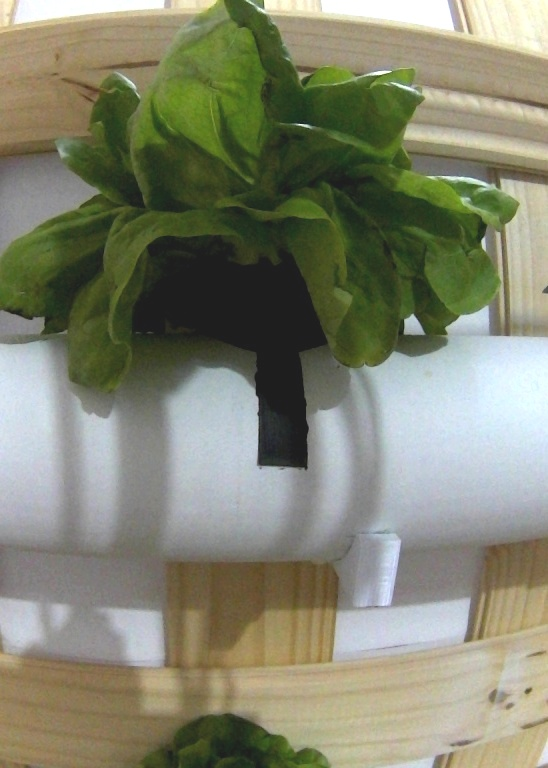
\includegraphics[width=0.6\textwidth]{imagenes/clasificador_1_original.jpg}
    \caption{Imagen RGB original}
\end{subfigure}
\hfill
\begin{subfigure}[b]{0.45\textwidth}
    \centering
    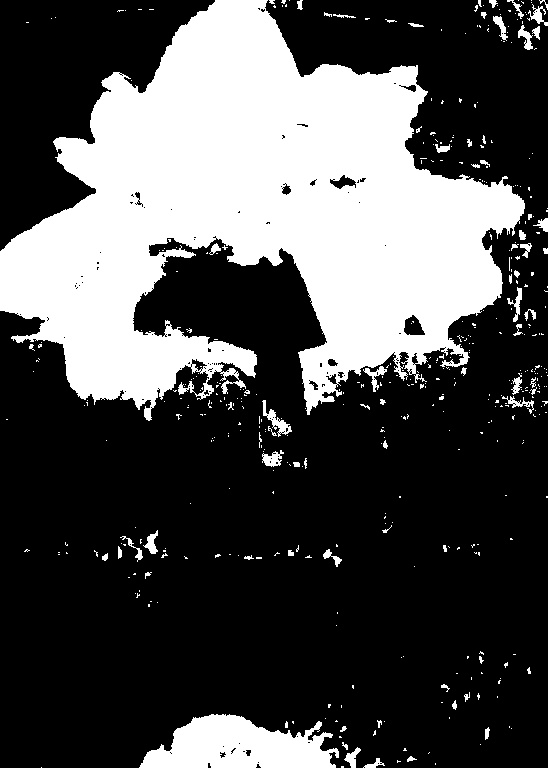
\includegraphics[width=0.6\textwidth]{imagenes/clasificador_2_verde.jpg}
    \caption{Máscara de vegetación verde}
\end{subfigure}
\caption{\textit{Etapa 1: Segmentación cromática en espacio HSV}}
\label{fig:clasificador_etapa1}
\end{figure}

Etapa 2: Refinamiento morfológico\\
\noindent
La máscara binaria presenta imperfecciones causadas por variaciones locales de iluminación y limitaciones del sensor. Se aplica una secuencia de operaciones morfológicas para refinarla:

\begin{itemize}[label=$\bullet$]
    \item \underline{Cierre morfológico}: Rellena huecos pequeños dentro de las regiones y conecta componentes próximos fragmentados.
    \item \underline{Apertura morfológica}: Elimina píxeles aislados y pequeñas protuberancias correspondientes a ruido.
\end{itemize}

Se emplea un elemento estructurante rectangular de 3×3 píxeles como compromiso entre eliminación de ruido y preservación de detalles relevantes.

\begin{figure}[H]
\centering
\begin{subfigure}[b]{0.48\textwidth}
    \centering
    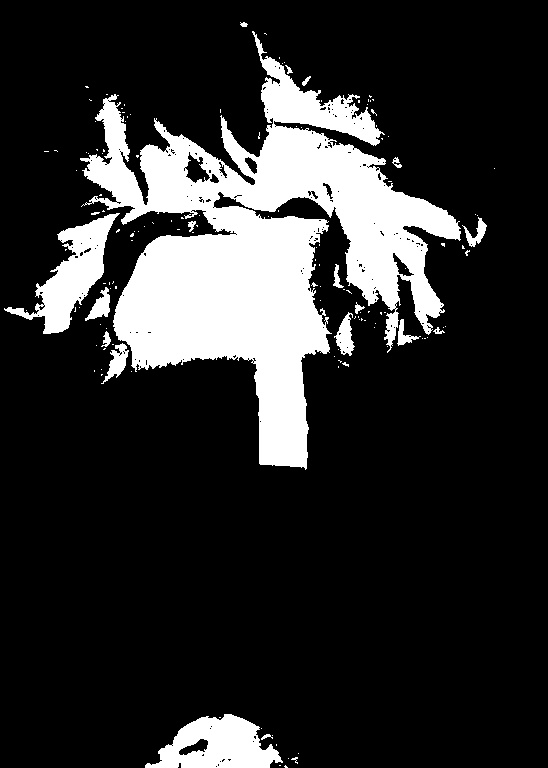
\includegraphics[width=0.6\textwidth]{imagenes/clasificador_3_negro.jpg}
    \caption{Máscara de regiones oscuras}
\end{subfigure}
\hfill
\begin{subfigure}[b]{0.48\textwidth}
    \centering
    
\includegraphics[width=0.6\textwidth]{imagenes/clasificador_4_combinado.jpg}
    \caption{Combinación verde + negro}
\end{subfigure}

\vspace{0.3cm}

\begin{subfigure}[b]{0.48\textwidth}
    \centering
    
\includegraphics[width=0.6\textwidth]{imagenes/clasificador_5_binario_final.jpg}
    \caption{Máscara binaria refinada}
\end{subfigure}
\hfill
\begin{subfigure}[b]{0.48\textwidth}
    \centering
    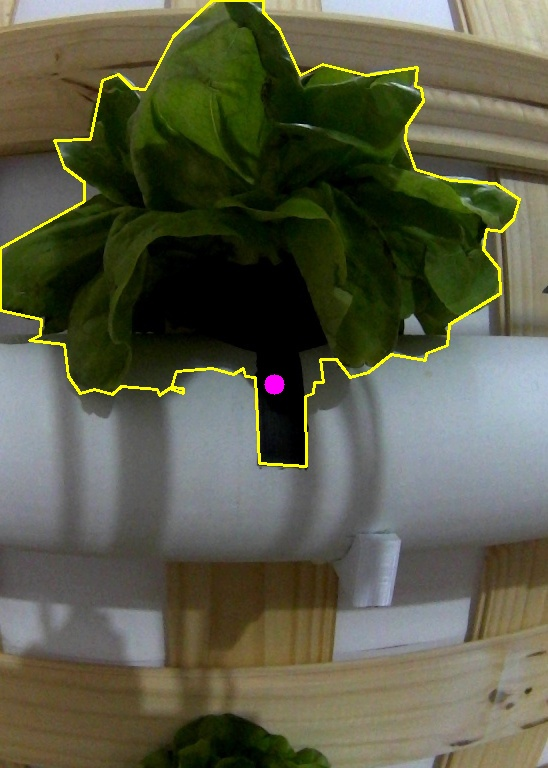
\includegraphics[width=0.6\textwidth]{imagenes/clasificador_6_contornos.jpg}
    \caption{Contornos finales detectados}
\end{subfigure}

\caption{\textit{Etapas del algoritmo de clasificación morfológica}}
\label{fig:clasificador_etapa2}
\end{figure}

Etapa 3: Detección y filtrado de contornos\\
\noindent
Sobre la máscara refinada se ejecuta detección de contornos que identifica las fronteras entre vegetación y fondo. Se emplea extracción de contornos externos únicamente, dado que las lechugas no presentan huecos internos relevantes.

Los contornos detectados se filtran por área mínima de 5000 píxeles, eliminando ruido residual y pequeñas sombras. De los contornos válidos, se selecciona el de mayor área bajo la hipótesis de que la lechuga constituye el objeto verde dominante en la escena.\\

Etapa 4: Clasificación por área\\
\noindent
El área del contorno seleccionado (en píxeles) constituye el descriptor empleado para clasificación. Se compara contra umbrales establecidos estadísticamente mediante análisis de muestras representativas. Áreas superiores al umbral indican lechuga madura lista para cosecha, mientras que áreas inferiores corresponden a plantas inmaduras o posiciones vacías.

Cuando no se detectan contornos válidos, el sistema clasifica la posición como vacía con alta confianza.


